\documentclass{article}

%packages
\usepackage{graphicx}
\usepackage{tikz}
\usepackage[utf8]{inputenc}
\usepackage{amssymb}

\begin{document}

\usetikzlibrary{automata,arrows, positioning}
\renewcommand{\contentsname}{Tabla de contenidos}

\begin{titlepage}
	\begin{center}
		
\includegraphics{./images/escudo.jpg}
	\end{center}
	\centering
	{\scshape\LARGE Complutense de Madrid \par}
	\vspace{1cm}
	{\scshape\Large Práctica Programación Evolutiva.\par}
	\vspace{1.5cm}
	{\huge\bfseries Segunda práctica. \par}
	\vspace{2cm}
	{\Large\itshape Raúl Torrijos \& Lukas Häring\par}
	%{\large Grupo 9\par}
	\vfill
	\vfill

% Bottom of the page
	{\large \today\par}
\end{titlepage}

\tableofcontents


\section{Introducción}
En esta práctica vamos a realizar una búsqueda de mínimos/máximos utilizando el Algoritmo Genético Simple. Los cromosomas pueden ser \textit{binarios}, basados en vectores de 0s y 1s para los genes, o \textit{reales}, basados en elementos Double (Valores de coma flotante). El algoritmo consta de 4 etapas (\textit{GeneticAlgorithm.java}): \textbf{evaluación}, dónde los cromosomas se evalúan, utilizando las funciones del guión como funciones de evaluación; \textbf{selección}, dónde se elige utilizando un criterio a los descendientes, en nuestra práctica, \textit{Ruleta}, \textit{Torneo Determinista} y \textit{Torneo Probabilista}; \textbf{Cruce}, de los candidatos elegidos, algunos se "mezclarán" (dos a dos) y crearán dos cromosomas distintos (dando mayor variabilidad); \textbf{Mutación}, muta aleatoriamente, en el caso de ser un cromosoma \textit{Binario}, bits del vector, si este es \textit{Real} existen dos tipos de mutación, una mutación de mínimo desplazamiento, se elige la bola más próxima al extremo y se genera un número aleatorio, o una mutación aleatoria, dónde un gen es reemplazado por otro valor distinto al que había.

En la práctica podemos seleccionar el elitismo, es decir, asegurarnos de que un subconjunto de cromosomas con mejor evaluación siempre son también descendientes puros (sin modificarse), y los \textit{n} peores serán reemplazados por los \textit{n} mejores.

\newpage

\section{Ejemplos}
Todos estos ejemplos (gráficos) se han realizado con los siguientes valores: un \textbf{Tamaño de población} de \textbf{100}; un \textbf{Número de generaciones} de \textbf{100}; un \textbf{60\%} de \textbf{Cruces}; un \textbf{5\%} de \textbf{Mutaciones} y una precisión para los cromosomas binarios de \textbf{0.0001}.
\subsection{Función 1}
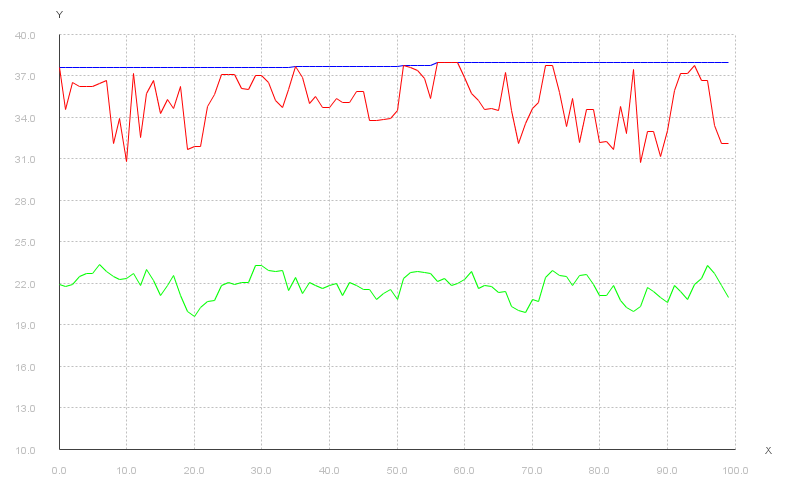
\includegraphics[scale=0.5]{./images/graph1_bin.png}
En general, hemos observado que el grado de evolución global es mucho mayor cuando el elitismo está activado. La calidad media generacional se ve mejorada notablemente.

Es la función más sencilla de aproximar, obteniendo valores (con elitismo activado) por encima del valor máximo de referencia del guión: 38.85026788587781 [x1: 11.625, x2: 5,725]
\subsection{Función 2}
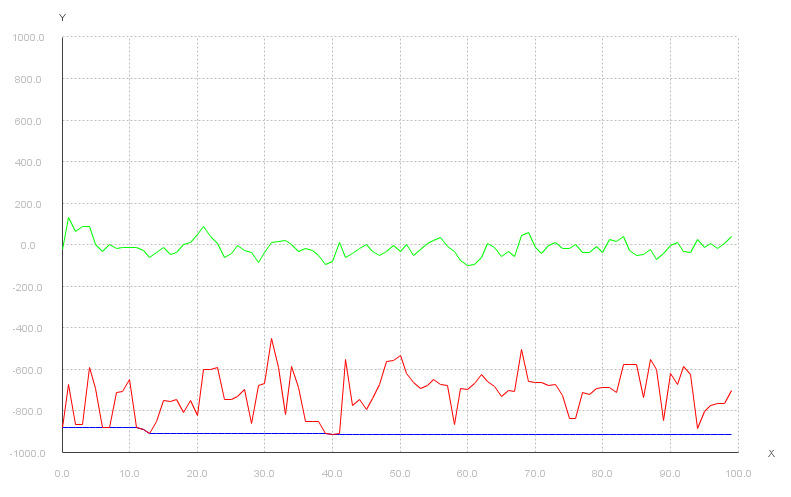
\includegraphics[scale=0.5]{./images/graph2_bin.png}
La aproximación al valor mínimo de la Función 2 es algo más costoso que el caso anterior. Sin elitismo obtenemos valores un tanto lejanos (en la mayoria de los casos entre -930 y -950). 

Necesitamos elitismo activado y 1000 generaciones para aproximarnos al mínimo de referencia: -959.6404193715668 [x1: 511.9999, x2: 404.2260]
\subsection{Función 3}
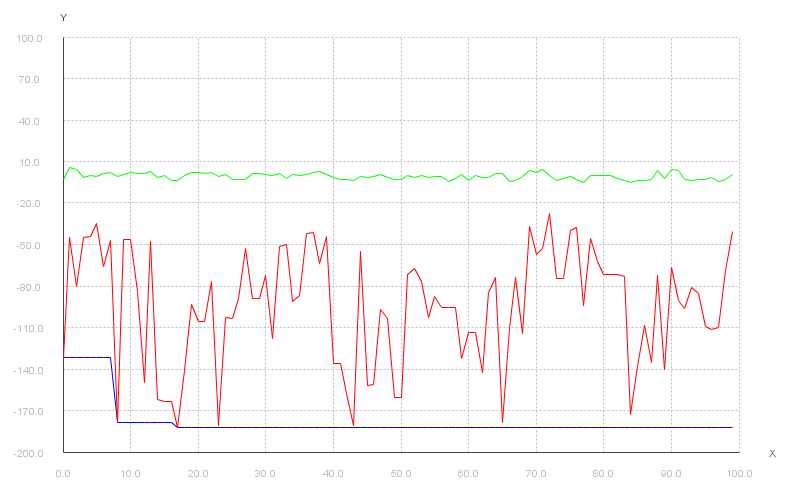
\includegraphics[scale=0.5]{./images/graph3_bin.png}
Con esta función los valores mínimos son alcanzados con mayor facilidad que con la anterior, con elitismo, son suficientes 100 generaciones (para una población de 100 individuos) para alcanzar un mínimo de 186.7302278988239 para [x1: 4.858, x2: -7.083]. Sin elitismo los valores mínimos varían entre -175 y -185 en la mayoría de los casos.
\subsection{Función 4}
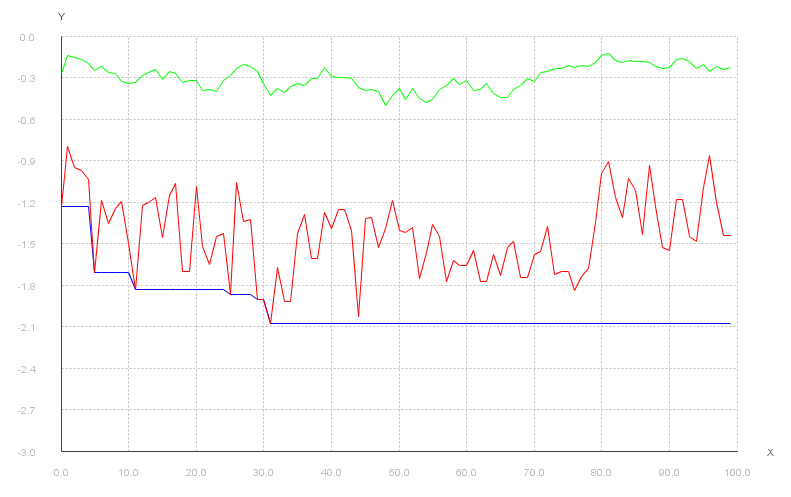
\includegraphics[scale=0.5]{./images/graph4_bin.png}
El número de argumentos de entrada para la Función 4 puede ser modificado directamente desde el panel de la aplicación.

Es la función más exigente de aproximar. A medida que le aumentamos el número de parámetros de entrada, la complejidad aumenta. Se recomienda utilizar con elitismo si se quieren obtener unos resultados cercanos a los del pdf. También hemos observado que para cuando el número de parámetros es 1, converge siempre al mismo valor: -0.8013033815890055 siendo [x1: 2.2028]. Por lo que pensamos que puede este ser el mínimo y no -1 (como indica el guión). 

También hemos observado un comportamiento similar con el caso de los cromosomas reales, pero cabe destacar el aumento de precisión a la hora de obtener, por ejemplo, el resultado para parametros=1, ya que es el mismo valor que con cromosomas binarios, pero los decimales menos significativos hemos observado que varían de una ejecución del algoritmo respecto a otra.
\subsection{Elitismo}
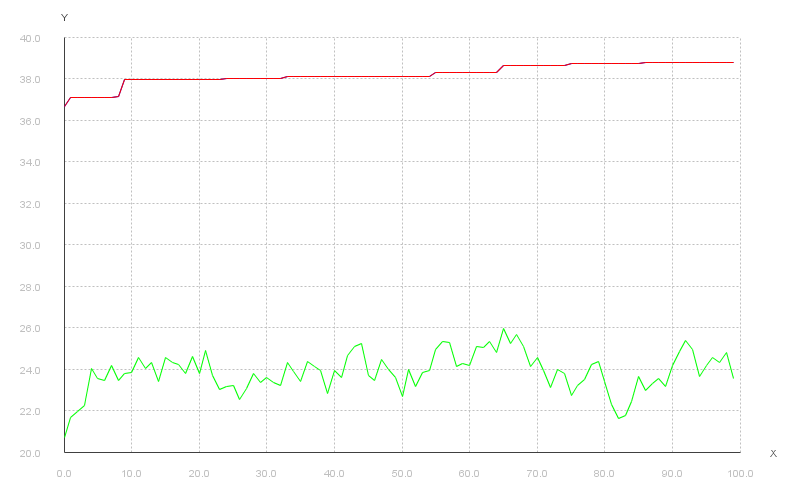
\includegraphics[scale=0.5]{./images/graph1_eli.png}
Como podemos ver, el mejor absoluto coincide con el mejor de la generación, esto es ya que siempre nos aseguramos que el mejor de la generación anterior siempre desciende o mejora, por lo que siempre va a estar ahí.
\end{document}
